\chapter{Exploiting mean reversion}\label{chap:jumps}

\begin{quotation}\noindent ``\emph{I can calculate the motions of the heavenly bodies but not the movements of the stock market}''. -- Sir Isaac Newton in 1768, after being wiped out in one of the many stock market crashes of his era.
\end{quotation}

Although financial markets are subject to discontinuities as described in Chapter 2, in some cases close interaction between financial instruments can serve to stabilise price movement over a period of time. In foreign exchange markets, for example, rates are expected to move in a self-consistent manner. If the Dollar-Yen and Euro-Dollar exchange rates change then the Euro-Yen rate should change accordingly. Delayed information flow and price inertia open up arbitrage opportunities. When the Dollar-Yen and Euro-Dollar markets are highly active the Euro-Yen rate may get out of line, but the expectation is that in due course it will revert to a value consistent with the other rates. This is a so-called \blacktext{\emph{triangular arbitrage}}. By buying and selling small lots throughout the day, high-frequency traders are able to exploit the mean-reverting property of exchange rates. 

For traders who trade larger lots with a longer time horizon, mean reversion cannot be exploited in this way. The profit would have been `locked in' after the 3rd currency pair is traded, but the trades will only be settled on two days later. So by the time the trade is settled, it doesn't matter whether the price has reverted or not, the profit has already been made. In my experience, a trader would do the reverse trades afterwards so that they don't need to commit the capital which they used for leveraging the trade before the settlement, due to credit risk, capital deposit or regulatory requirements such as BASEL II.


More generally and in a less mechanical manner when the prices of two positively correlated assets diverge temporarily, we will expect one of the prices to revert to a price consistent with the other, over some period of time. A classical strategy is \emph{pairs trading} where a portfolio consisting of a weighted combination of two assets is traded. Profit is determined by the choice of weights in the linear combination as well as the market timing to enter and close a position. The choice of weights involves the measurement and interpretation of correlation and volatility. Adaptive estimates of these quantities can be used with the dynamic linear model of Section \ref{sec:dynamicLM} to predict the return for an asset that has not recently traded. The predicted value is then compared with the quoted price in the order book to take advantage of any temporary anomaly and to trade profitably relying on subsequent mean reversion to remove the anomaly \blacktext{and the cost of the trade}. See Chapters \ref{chap:volatility} and \ref{chap:covolatility}, for further discussion of volatility and correlation estimation in financial data.    

Hunting for mean reversion lies at the heart of successful high frequency trading. Proprietary noise traders exploit pricing inefficiencies across securities and other asset classes, both locally and globally. In local trading on a specific exchange, transient price anomalies can be expected to disappear rapidly as the force of market opinion returns the price to its former level. If the price is low, for example, this is an opportunity to buy with the prospect of selling later as the price reverts. By trading rapidly, small gains can be accrued on such events. 
%This is described in Section \ref{sec:optimalTrading}. 

At a global level, high-frequency traders exploit low-latency computer networks to access geographically separated markets. They determine the price they are prepared to quote to other market participants bearing in mind lead-lag delays as pricing information flows around the world. Stale prices on exchanges that are remote from the principal sources of price formation can be expected to revert to a more generally accepted norm over a short period of time.  This is studied in Chapter \ref{chap:lagCorrelation}. 




The high-frequency trading arms race is a consequence of continuous-time trading on electronic financial exchanges. That is, under the current continuous limit order book market system, it is possible to buy, sell, and post orders for exchange-traded financial instruments extremely rapidly at any instant during the trading day. 
%For example, there are approximately 215,000 quote updates per second on the New York Stock Exchange. 
The appearance of multiple electronic trading venues has led to an increase in frequency and volume of transactions and order flow. The objective of all traders, whether an algorithmic or a human trader, remains the same: to buy low and sell high. 

A typical high-frequency trading algorithm runs on a sub-millisecond time scale and has very short portfolio holding periods, usually well under five seconds and frequently less than one second. Large amounts of data are processed every millisecond and there is a requirement is to act rapidly to these data as the profitability of the signals in the market decays very quickly. Substantial investments have been made by the high-frequency trading community utilising custom built fibre-optic, microwave and millimetre-wave networks and dedicated hardware based on field programmable gate arrays \citep{leber2011high}. Even with these investments, the need for speed prioritises statistics that can be computed in linear time and updated recursively. 

In this chapter we focus on recursive methods for rapid trading and the exploitation of mean reversion. The applied forecasting world has a long history of using recursive methods to predict future outcomes. Basic kernel-based methods are described in Section \ref{sec:fastTradingAlgo} and the extension to recursive linear regression in Section \ref{sec:EWLS}.  The classic filtering methods of the dynamic linear model (DLM) and Kalman filter are motivated in a financial context in Section \ref{sec:dynamicLM}.  The close connection between the Kalman filter and the exponentially weighted moving average forecast is illustrated in Section \ref{sec:EWMAKalman} for completeness. 

News announcements can produce major disruptions to the market, as described in Section \ref{sec:disrupt}. A fundamental question is whether prices will revert to their earlier values, either in real or absolute terms, and whether historical correlations under benign conditions can be relied upon to persist in a new and unexplored trading environment. Modelling of these special events needs to take account of the influence of external factors as well as the sensitivity of dynamic models to initial conditions.  This is briefly discussed in Section \ref{sec:disrupt} -- although it is not the main focus of the high-frequency trading community.  
\section{Forecasting, filtering and time change}\label{sec:forecast}

A basic concept in finance is that of the underlying fair value of an asset. In practical terms, when looking for profitable opportunities, traders compare the currently available price with their estimate of the fair value at some future time point. When the current price is lower than their estimate they buy and when it is higher they sell. The underlying belief is that the price will revert to their estimated fair value. 

In estimating future values based on the past, practitioners can call on a range of forecasting methods drawn from a wide variety of disciplines.  Broadly speaking the methods are of two types: those based on mathematical modelling often with an underlying Bayesian philosophy and those based on practical experience in Operations Research and other applied fields.  We will refer to them as \emph{model-based} and \emph{traditional} forecasting methods, respectively.  \citet{shephard2015martingale} uses the term `non-model' to describe traditional methods. 

\subsection{Traditional forecasting}
Traditional forecasting has a long history going back to the work of Brown and Holt in the 1950s. Holt's  1957 report to the Office of Naval Research is reprinted in \citet{holt2004forecasting} and Brown's contributions are recounted in his historical review \citep{brown2004smoothing}. The exponentially weighted moving average (EWMA) emerged at that time as an expedient way of computing a moving average providing `savings in data storage over moving averages' owing to the recursive nature of its calculation \citep{gardner2006exponential}. The EWMA can be used as a forecast of future values when no change is expected. 

In general, the quality of a traditional forecast is judged by empirical performance and any parameters involved optimised accordingly. Similarly, extensions aimed at forecasting trends can be assessed by their performance in practice.  In other words, model assumptions are not emphasised and judgements about the adequacy of the method are entirely empirically based. One of the benefits of this practical approach is that considerable flexibility can be introduced into forecasting formulas.  For example, \citet{trigg1995exponential}  developed a popular adaptive version  of the EWMA. For other practical modifications, extensions and variants of the EWMA, see \citet{brown2004smoothing} and \citet{gardner2006exponential}. The disadvantage of traditional methods is that it is difficult to find guidance on which method to use, so each new application has to be approached on a trial and error basis. 

\subsection{Model-based forecasting}
By contrast, in this formulation a model is assumed for an underlying unobserved process and a specific model is introduced for the observation process. The objective is to recover the underlying process after filtering out the noise. Basic filtering theory with emphasis on stochastic differential models is covered in \citet{davis1997linear} and \citet{oksendal2003stochastic}, for example.  In finance the simplest model of price movement on a logarithmic scale has Brownian motion as the underlying process with independent observational noise. We will assume that price is always measured on a logarithmic scale, use `log-price' to denote the logarithm of the price from now on. In practice the model is a poor fit to observations particularly with high-frequency data. To remedy this the model has been extended to allow stochastic evolution of the infinitesimal variance in the underlying diffusion, i.e.\ the introduction of \emph{stochastic volatility}. \citet{shephard2015martingale} provides historical background  with further extensions, and modern developments. For a comprehensive review of filtering and forecasting in finance with particular focus on statistical techniques that have been used to accommodate stochastic volatility, see the compendious \citet{bauwens2012handbook}.

\subsection{Time change}\label{sec:timechange}
Before discussing forecasting methods, it is important to consider the nature of time in a high-frequency trading environment. We cannot emphasis more strongly the importance of this topic in determining the fundamental time-scale for the analysis of high-frequency trading data. It is well known that price fluctuations occur in  bursts, as a result of highly competitive trading interaction. These changes in price volatility can be explained by stochastic volatility models. In the simplest case, log-price is modelled as Brownian motion with stochastic infinitesimal variance.  Since the volatility is not constant, price changes over a fixed period of time are no longer normally distributed and may be heavy-tailed, as observed empirically. 

In an alternative formulation, as has been pointed out by \citet{clark1973subordinated}, the price process can be thought of as evolving on a non-uniform time scale.  With a suitable time change, the volatility is constant and standard Brownian motion can be reconstructed. In other words, if the underlying price $X(t)$ is modelled as
$$
dX(t) = \sigma(t) dB(t),
$$
where $B(t)$ is standard Brownian motion, then  
\begin{equation}U(t) = X(T(t)),\quad  t \geqslant 0
\end{equation} is standard Brownian motion when $T(t) = \int_0^t 1/\sigma^2(u) du$. For a discussion of the necessary conditions for this to hold, see for example \citet{veraart2010timechange}. 

When only the price of the asset is available and the underlying volatility is unknown, the representation via time-change is of limited practical use. However \citet{ane2000order} have shown that approximations to $T(t)$ can be obtained by using other information provided in modern high-frequency market data. In particular they show that an \emph{activity time-scale} can be constructed as an affine function of the cumulative transaction count and that with this time change, log-price increments are no longer heavy tailed and are well approximated by Gaussian distributions. See also \citet{easley1992time}. To a certain level of approximation they argue importantly that on the activity time-scale, volatility can be considered to be constant.  In the same paper they consider an earlier proposal by \citet{clark1973subordinated} to use the cumulative \emph{volume} of trade as a time scale but show that this has inferior properties.   

High-frequency traders can choose to construct their forecasts on physical time, trading activity time or more elaborate time scales involving cumulative activity as measured by cancellations, modifications and the arrival of new orders.  The choice will be determined by the empirical performance of the forecasting or filtering methods they adopt.      
   

\section{Marked point datasets}
Electronic exchanges produce streams of data in packets tagged by timestamps and values.  The timestamps and values are both discrete.  If we consider the arrival of such a packet as an event, the data have the structure of observations from a marked point process. There is an extensive literature on the modelling of marked point process with early applications to the statistical analysis of earthquake data where events correspond to earthquakes at specific times and the marks describe characteristics of the seismic activity. See \citet{cox1980point,ogata1988statistical,daley2007introduction} and the references therein.  

A marked point dataset is a sequence of events at distinct times $t_1,t_2,\dots,t_n$ with associated values $Z_1,Z_2,\dots,Z_n$ at these times. The data can be represented by the step function
\begin{equation}\label{eq:pricestep}S(t) = \sum_{i:t_i \leqslant t} Z_i, \quad  t \in R,\end{equation}
the cumulative sum of the values at or before time $t$.

The simplest example is the counting function $N(t), t \in R$,  which counts the number of events that have occurred at or before $t$.

In financial application, we may be interested in comparing two counting functions, for example the number of {\em given} trades and the number of {\em paid} trades over a period $(0,t)$. If $N_p(t)$ is the number paid and $N_g(t)$ is the number given then $N_p(t) - N_g(t)$ is a marked point dataset where $t_1,t_2,\dots,t_n$ are the trade times and $Z_i = 1$ at time $t_i$ if the trade is paid and $Z_i = -1$ if it is given, $i=1,2,\dots,n$.  

Similarly if  $V_p(t)$ is the cumulative volume of paid trades over the period $(0,t)$ and $V_g(t)$ is the cumulative volume of given trades, then the net volume of trade, $V_p(t) - V_g(t)$, is a marked point dataset with $Z_i$ equal to $V_i$ or $-V_i$ depending on whether the traded volume, $V_i$, is paid or given.

Finally, the bid, ask or mid log-price of an asset can be thought of as marked point dataset where $t_1,t_2,\dots $ are the times at which prices have changed and $Z_1,Z_2,\dots$ are the log-price changes, positive or negative.

Trades are the simplest events in data from an electronic exchange. When a trade occurs, the exchange publishes the time of the trade along with the price and quantity trade. The price and quantity as a pair are the mark associated with the trade.  Events involving new quotations to buy or sell, modifications of existing orders and cancellations produce more complicated marks.  These form the fundamental `ticks' of market data. In some cases the events will result in changes to the best prices offered to buy and sell.  When a quoted price changes it persists until altered by subsequent events. An order associated with the price is said to be resting and is available for trade until removed. Of course, alterations to prices deeper in the order book do not affect the best prices, but nevertheless this deeper information is published by the exchange and may indicate changes in market sentiment and the direction in which the market will move.  

\section{Recursively calculated forecasts}\label{sec:fastTradingAlgo}
A first step in the exploitation of mean reversion is to establish a starting point. In practice this involves smoothing recent values using an appropriate moving average. As a specific example we suppose the data are observations, $X(t) = x(t)$ of the exchange quoted log-price -- taking `price' to be mid-price, the average of the bid and ask prices. Let $\{t_k\}$ be the times  at which prices are updated and write $x_k = x(t_k)$ for notational convenience.

We consider a class of kernel-based smoothers that include the exponentially weighted moving average as a special case. Choosing the kernel is one of the main difficulties in statistical analysis. In practice, high frequency traders try out different kernels. See \citet{brown2004smoothing} for an introduction to the extensive traditional forecasting literature.
\subsection{Kernel based moving averages}
Throughout this Chapter, we will use the word `kernel' to refers to any integrable function $K$ on $[0,\infty)$ such that 
\begin{equation}\label{eq:kernelDef}
\int_0^\infty K(u) du = 1.
\end{equation}
Note that $K$ is not required to be non-negative.

The kernel can be used to produce a moving average of the quoted log-price $x(t), t \in R$, as follows:
$$ \hat{\nu}(t) = \int_{-\infty}^t K(t-u) x(u) du.$$
 
For the exponential kernel, $K(x) = \tau^{-1}e^{-x/\tau}, x \geqslant 0$, we define the \emph{exponentially weighted moving average} (EWMA) of $x(t), t \in R$ to be
$$ \hat{\nu}_1(t) = \int_{-\infty}^t \tau^{-1} e^{-(t-u)/\tau} x(u) du.$$
Note in the traditional forecasting there are other variants of the EWMA \citep{gardner2006exponential}.
Since $x(t)$ is a step function with value $x_k$ on the interval $[t_k,t_{k+1})$ we have
\begin{align}\label{EWMAint} \hat{\nu}_1(t) &= x_k \int_{t_k}^t \tau^{-1} e^{-(t-u)/\tau} du + \sum_{i \leqslant k}x_{i-1} \int_{t_{i-1}}^{t_i} \tau^{-1} e^{-(t-u)/\tau} du \nonumber\\
&= x_k \left(1 - e^{-(t-t_k)/\tau}\right) +  \sum_{i \leqslant k}x_{i-1} \left(e^{-(t-t_{i})/\tau} - e^{-(t-t_{i-1})/\tau}\right),
\end{align}
where $t_{k} < t \leqslant t_{k+1}$.

At event times we get the EWMA recurrence,
\begin{align}\label{eq:EWMArecurrence}
\hat{\nu}_1(t_{k+1}) &= \int_{-\infty}^{t_{k+1}} \tau^{-1} e^{-(t_{k+1} -u)/\tau} x(u) du \nonumber \\
&= e^{-\Delta_k/\tau} \int_{-\infty}^{t_k} \tau^{-1} e^{-(t_k -u)/\tau} x(u) du + 
x_k \int_{t_k}^{t_{k+1}} \tau^{-1} e^{-(t_{k+1} -u)/\tau} du \nonumber \\
&= e^{-\Delta_k/\tau} \hat{\nu}_1(t_{k}) + (1-e^{-\Delta_k/\tau}) x_k,
\end{align}
where $\Delta_k = t_{k+1} - t_{k}$, and we have used the fact that $x(u)$ is a step function with constant value $x_k$ for $t_k \leqslant u < t_{k+1}.$

For an intermediate time $t$ between $t_k$ and $t_{k+1}$ we have 
\begin{equation}\hat{\nu}_1(t) = e^{-(t-t_k)/\tau} \hat{\nu}_1(t_{k}) + (1-e^{-(t-t_k)/\tau}) x_k.\end{equation}
Note that when $\{t_k\}$ are equally spaced, i.e.\ $\Delta_k = \Delta$, from expression \eqref{EWMAint} we have the simplest form of the EWMA
\begin{align} \hat{\nu}_1(t_{k+1}) &= (1-e^{-\Delta/\tau}) \sum_{i \leqslant k} x(t_i)e^{-\Delta(k-i)/\tau}\nonumber\\
&= (1-\lambda) \sum_{i \leqslant k} x_i \lambda^{(k-i)}, \quad \text{where $\lambda = e^{-\Delta/\tau}$}.
\end{align}

More general kernels are provide by the gamma family. Gamma kernels are non-negative with flexible shape depending on a parameter $\alpha$. The gamma kernel is
$$ K(x) = x^{\alpha-1} e^{-x/\tau} \tau^{-\alpha}/\Gamma(\alpha), \quad \tau > 0, \quad 
\alpha > 0,$$
giving the moving average
$$ \hat{\nu}_{\alpha}(t) = \int_{-\infty}^t (t-u)^{\alpha-1} e^{-(t-u)/\tau} \tau^{-\alpha}/\Gamma(\alpha)x(u) du.$$
The case $\alpha=1$ this is the exponential kernel. When $\alpha > 1$ the moving average puts less emphasis on values immediately prior to $t$.

Moving averages based on the gamma kernel can be updated recursively. For example, when $\alpha = 2$ we have
\begin{align*}
\hat{\nu}_2(t_{k+1}) &= \int_{-\infty}^{t_{k+1}} \tau^{-2}(t_{k+1}-u) e^{-(t_{k+1}-u)/\tau} x(u) du\\
&= \int_{-\infty}^{t_k} \tau^{-2}(\Delta_k +t_k -u) e^{-(t_{k+1}-u)/\tau} x(u) du + x_k\int_{t_k}^{t_{k+1}}\tau^{-2} e^{-(t_{k+1}-u)/\tau}du\\
&= e^{-\Delta_k/\tau}\left(\frac{\Delta_k}{\tau}\hat{\nu}_1(t_k)  +\hat{\nu}_2(t_k)\right) + x_k\left(1 - \frac{\Delta_k}{\tau}e^{-\Delta_k/\tau} - e^{-\Delta_k/\tau}\right), 
\end{align*}
a recursion in terms of $\hat{\nu}_1$ and $\hat{\nu}_2$.

\subsubsection*{What does $\hat{\nu}_\alpha$ estimate?}
Up until now, as in much of the traditional forecasting literature, we have made no distributional assumptions about $x(t)$. Nevertheless, if we assume that $x(t)$ it is a realisation of a random process $X(t)$ then by linearity
\begin{equation}\label{eq:zerolag}
E[\hat{\nu}_\alpha(t)] = \int_{-\infty}^t \frac{\tau^{-\alpha} (t-u)^{\alpha-1}}{\Gamma(\alpha)} e^{-(t-u)/\tau}\nu(u) du,
\end{equation}
where $\nu(u) = E[X(u)]$.

If we suppose that $\nu(u)$ is locally linear around time $t$, i.e.\ $\nu(u) \approx b_0 + (u-t)b_1$ then from \eqref{eq:zerolag}
$$ E[\hat{\nu}_1(t)] \approx b_0 - b_1 \tau \quad \text{and} \quad E[\hat{\nu}_2(t)] \approx b_0 - 2 b_1 \tau.$$
In other words, $\hat{\nu}_1(t)$ estimates the expected value of $X$ at time $t-\tau$ and $\hat{\nu}_2(t)$ at $t-2\tau$.  

Putting these together, we see that the expected value at time $t$ is estimated by $2 \hat{\nu}_1(t) - \hat{\nu}_2(t)$, the so-called {\em zero lag forecast} \citep{brown2004smoothing}.  

The zero lag forecast is also a kernel estimate with kernel
$$K(u) = \frac{e^{-u/\tau}}{\tau^2} (2 \tau - u), \quad u \geqslant 0.$$
Note that $K(u)$ is negative when $u> 2 \tau$ but tends to zero as $u \to \infty$. Furthermore 
$$[2 + \tau^{-1}(s-t)]\hat{\nu}_1(t) - [1 + \tau^{-1}(s-t)]\hat{\nu}_2(t)$$ estimates the expected value at some time $s$ in the future, $s>t$ and the local slope, $b_1$, is estimated by $\tau^{-1}(\hat{\nu}_1(t) - \hat{\nu}_2(t)\blacktext{)}$. 

\subsection{Detecting changes with an EWMA}
Suppose as previously that $x(t)$ is the quoted log-price of an asset. To assess the difference between the current log-price and earlier log-prices,  and hence detect changes and exploit mean reversion, we can look at the current log-price minus a kernel-based moving average of the log-price, for example 
$$x(t) - \hat{\nu}_1(t).$$
Alternatively, in this case, we can look at the Stieltjes integral
$$\hat{\mu}_1(t) = \int_{-\infty}^t \tau^{-1} e^{-(t-u)/\tau} dx(u),$$
where exponential weights are applied to the \emph{increments in the log-price}.
It turns out that the two approaches are essentially the same since, integrating by parts, we have 
\begin{align*}
\hat{\mu}_1(t) &= \int_{-\infty}^t \tau^{-1} e^{-(t-u)/\tau} dx(u) \\
&= -[x(t) - x(u)]\tau^{-1}e^{-(t-u)/\tau}|^{u=t}_{-\infty} + \int^t_{-\infty} [x(t) - x(u)]\tau^{-2}e^{-(t-u)/\tau} du\\
&= \tau^{-1}[x(t) - \int_{-\infty}^t x(u) \tau^{-1} e^{-(t-u)/\tau} du] \\
&= \tau^{-1}[x(t) - \hat{\nu}_1(t)].
\end{align*}
The only difference being the term $\tau^{-1}$ that converts the log-price change into change per unit time.

\subsection{Iterating EWMAs}
EWMAs can be iterated, i.e.\ the EWMA of an EWMA can be calculated. We can show that this does no more than produce a linear combination of two EWMAs. Write $\hat{\nu}_1(t,\tau_1)$ for the EWMA of $X$ using half-life parameter $\tau_1$. The EWMA of this EWMA using parameter $\tau_2 \neq \tau_1$ is then
\begin{align*}
\int_{-\infty}^t \tau_2^{-1} e^{-(t-u)/\tau_2}\hat{\nu}_1(u,\tau_1) du 
&= \int_{-\infty}^t \tau_2^{-1} e^{-(t-u)/\tau_2}\int_{-\infty}^u \tau_1^{-1} e^{-(u-w)/\tau_1}x(w) dw du \\
&= \int_{-\infty}^t (\tau_1 \tau_2)^{-1}e^{-t/\tau_2 + w/\tau_1}\int_{w}^t e^{-u(1/\tau_1 - 1/\tau_2)} du dw \\
&= \frac{\tau_2}{\tau_2-\tau_1} \hat{\nu}_1(t,\tau_2) - \frac{\tau_1}{\tau_2-\tau_1} \hat{\nu}_1(t,\tau_1).
\end{align*}

\subsubsection*{What does the difference between two EWMAs estimate?}
Suppose that $E[X(u)] = \nu(u)$ is locally linear around time $t$ so that $\nu(u) \approx b_0 + (u-t)b_1$ as before, then
$$E[\hat{\nu}_t(t,\tau_1)] \approx b_0 - b_1 \tau_1 \quad \text{and} \quad E[\hat{\nu}_t(t,\tau_2)] \approx b_0 - b_1 \tau_2.$$
It follows that $b_1$, the slope of the local trend, is approximated by
$$ b_1 \approx \frac{\hat{\nu}_t(t,\tau_1) - \hat{\nu}_t(t,\tau_2)}{\tau_2-\tau_1}$$
and the zero-lag approximation to $b_0$ is
$$ b_0 \approx \frac{\tau_2 \hat{\nu}_t(t,\tau_1) - \tau_1 \hat{\nu}_t(t,\tau_2)}{\tau_2-\tau_1}.$$
Combinations of these quantities give projections to future time points.
\subsection{Estimation of parameters}
In practice, parameters in a forecasting formula are determined by assessing the performance of the forecast. If the forecast aims to predict the price at some future point in time, then the quality of the forecast can be tested with historical data and the parameters adjusted accordingly. \citet{taylor2004smooth} notes that `The
literature generally recommends that the smoothing parameters should be estimated from the
data, usually by minimising the sum of \emph{ex post} 1-step-ahead forecast errors'. These are the recommendations in \citet{gardner2006exponential}. In practice historical data is split into two sets: the `in-sample' and the `out-sample'.  The method is optimised using the in-sample data and then performance is checked with the out-sample.  

A typical experiment would be to take several days of market data and at each time point compare the EWMA smoothed price with the current price of the asset. This difference is then compared with the future return of the asset over say 30 seconds, i.e.\ the difference between the price 30 seconds ahead and the current price.  This is repeated for each time point. The objective is to predict the future return from the EWMA difference.   When the predicted future return is positive, this is an opportunity to buy and when it is negative an opportunity to sell. There are parameters in the gamma-kernel smoother, $\alpha$ and $\tau$ and parameters in the prediction procedure. All of these are then optimised to achieve the maximum empirical profit in the historical data. The approach is model-free and the optimal parameters are determined empirically.   
\subsection{Exponentially weighted least squares}\label{sec:EWLS}
Recursive smoothing and forecasting methods can be extended to include external factors. By formulating the problems as exponentially weighted least squares, recursions can be established for the regression parameters.  There is a long history of this algorithm in tracking time-varying parameters \citep{brown2004smoothing}. 

Again using quoted log-price $y(t)$ as an example, let $y_j = y(t_j)$ where $t_j$ are the times of log-price increments. Suppose that at time $t_j$ we have available a vector of explanatory variables $\bfa_j$, $j=1,2,\dots,k$. The objective is to predict $y_{k}$ based on $\{y_i,i \leqslant k-1 \}$ and $\bfa_k$. In high-frequency trading applications, the elements of $\bfa_k$ might include measurements such as bid-ask spread, bid-ask volume imbalance, number of quotes, trades during the immediate past and other characteristics of the order book, i.e.\ the difference between the amount available to buy and to sell at the best price. For brevity we will only consider the case where $\{t_j\}$ are equally spaced. 

The exponentially weighted least squares estimate of the regression coefficients $\beta_k$ at the time of the $k$th event is defined to be
\begin{equation}\label{eq:RLSobjective} 
\hat{\beta}_k= \underset{\beta}{\text{argmin}} \sum_{j=0}^k (y_j  - \bfa_j^T \beta)^2 \wlambda^{k-j} .
 \quad \text{where $0 < \wlambda < 1$}.
\end{equation}


From \eqref{eq:RLSobjective}, differentiating the right hand side w.r.t. $\beta$ gives $\hat{\beta}_k$,
$$\hat{\beta}_k = \left(\sum_{j=0}^k \bfa_j \bfa_j^T \wlambda^{k-j} \right)^{-1} \sum_{j=0}^k \bfa_j y_j \wlambda^{k-j} = R_k^{-1} P_k,$$
where $R_k$ and $P_k$ can be calculated recursively by
\begin{align}\label{sec:recursion}
R_k &= \wlambda  R_{k-1} + \bfa_k \bfa_k^T, \qquad R_0 = I \nonumber  \\
P_k &= \wlambda P_{k-1} + \bfa_k y_k, \qquad P_0 = \bfa_0 y_0.
\end{align}
If $R_k $ is nonsingular, then $\hat{\beta}_k$ is the unique solution for predicting $\tilde{y}_{k}$.
Using a matrix inversion formula \citet{rao2009linear}, the inverse of $R_k$ can also be calculated recursively as
$$R_k^{-1} = \frac{1}{\wlambda} \left\{I - \mathbf{v}_k \bfa_k^T \right\}R_{k-1}^{-1},$$
where 
$$ \mathbf{v}_k = R_{k-1}^{-1}\bfa_k/(\wlambda + \bfa^T_k R_{k-1}^{-1} \bfa_k).$$ 


In practice, there are difficulties with the  $R_{k}^{-1}$ recursion since $ R_{k}$ may be near-singular during patches of data where the feature vectors change very little and are highly correlated. The method can \textcolor{black}{be} stabilised by the addition of ridge terms \textcolor{black}{$\lambda_k$} on the diagonal of $R_k$ from time to time before inversion, for example when indicated by the condition number of the matrix $R_k$.
\textcolor{black}{
	\begin{align}\label{sec:ridge}
	R_k^{ridge} = R_k + \lambda_k I \nonumber.
	\end{align}
}

This makes $R_k^{ridge}$ nonsingular, even if $R_k$ is not of full rank, and was the main motivation for ridge regression when it was first introduced by \citet{hoerl1970ridge}.

Ridge regression shrinks the estimated coefficients by imposing a penalty on the residual sum of squares. Here $\lambda_k \geq 0 $ is a tuning parameter which controls the strength of the penalty term. As such, it has the affect of shrinking the regression coefficients towards zero. This introduces some bias, but can greatly reduce the variance, resulting in a better mean-squared error. Large $\lambda_k$ means more shrinkage, and so we get different $\hat{\beta}_k$ for different values of $\lambda_k$. Choosing an appropriate value of $\lambda_k$ is hard but normally is done by 5-fold cross-validation in high-frequency trading analysis.

Ridge regression performs particularly well when there is a subset of true coefficients that are small or even zero. It does not do as well when all of the true coefficients are moderately large; however, in this case it can still outperform linear regression. See \citet{trevor2001elements}.

The prediction of the next value $y_k$, given $\bfa_1,\dots,\bfa_k$ and $y_1,\dots,y_{k-1}$, is then given by
$$\tilde{y}_{k} = \bfa^T_k \hat{\beta}_{k-1}.$$
The estimated coefficients $\{\hat{\beta}_k\}$ are updated by
$$
\hat{\beta}_k = \hat{\beta}_{k-1}  + R^{-1}_k \bfa_k (y_k - \tilde{y}_{k}). 
$$
Again it is worth emphasising that  estimates obtained by exponentially weighting do not in general coincide with the optimal values derived from the Kalman filter of Section \ref{sec:updateKF}. They are convenient approximations that can be rapidly calculated. For further details and extensions to forward forecasting, see \citet{brown2004smoothing}.


\subsection{Moving averages for volatility and covolatility}\label{sec:MAvolcovol}
In the interest of speed, it may be possible more generally to replace a locally defined linear statistic by a recursively defined approximation. As we shall see in Chapters \ref{chap:volatility} and \ref{chap:covolatility}, the realised volatility and the ZHY estimate of covolatility both have a linear form. These quantities can be expected to vary throughout the trading day. As a consequence local estimates defined in a window of time may be appropriate. 

In essence, the idea is to replace the windowed sum  $\sum_{i=n-m+1}^n a_i x_i$ ($m$ fixed)  for arbitrary sequences $(x_i)$ and $(a_i)$ with
$$\hat{h}(n) =  \sum_{i\leqslant n}  \wlambda^{n-i}  a_i x_i, \quad 0< \wlambda < 1$$
which can be calculated with the recursion 
\begin{equation}\label{eq:recursevolcovol}\hat{h}(n+1) = \wlambda \hat{h}(n) + a_{n+1} x_{n+1}.\end{equation}   
 
\section{Dynamic linear models}\label{sec:dynamicLM}
\blacktext{A simple strategy to profit from mean-reversion is to place thresholds at one standard deviation above and below the estimated mean-reverting level. Buy one unit of the portfolio if the low threshold is hit or sell one unit of the portfolio if the high threshold is hit. To take profit from the strategy is to close the position when the value of the portfolio is within a small interval of the mean-reverting level. This naive strategy is not guaranteed to make profit and in fact the trader may enter a long or short position which never reverted back to the inner band by the end of the trading horizon. This will induce potential losses into the strategy as the trader tries to flatten his or her position. The wider the trigger thresholds, the less likely it is to end up flat.}

To give some idea of the principles applied in successful trading we start by looking at an elegant technical paper by \citet{thompson2002optimal} who develops optimal strategies for trading an asset driven by a hidden Markov process. \blacktext{He presents an intuitive derivation by viewing the optimal trading problem as a pair of simultaneous optimal stopping problems.} We then go on to consider how to turn such ideas into practical trading strategies in terms of dynamic linear models. \blacktext{In this context, the trader will make a single round trip trade and there is no terminal time horizon.}

In the simplest case, Thompson assumes the efficient log-price $\breve{X}(t)$ is an Ornstein-Uhlenbeck process with
$$ d\breve{X}(t) = -\gamma \breve{X}(t) + \sigma dB(t),$$
where $B(t)$ is standard Brownian motion \blacktext{ and $\gamma > 0$} is the reversion rate. We annotate $X$ as $\breve{X}$ to distinguish the observable log-price from the hypothetical efficient log-price.

To take account of the cost of \emph{paying the spread} in real life aggressive trading, each trade incurs a transaction cost of $c/2 > 0$. The efficient log-price is assumed to be observable without error. The trader can only hold either 1 or 0 units of the asset.

\subsection{Optimal trading}\label{sec:optimalTrading}
Thompson shows that the optimal strategy to maximise long-term profit is to buy when $\breve{X}(t)$ hits a low threshold and sell when it hits a high threshold, This is perhaps not surprising but Thompson gives the optimal thresholds precisely as $\pm b/\gamma$ where 
$$ 2b - \gamma c = 2 e^{-b^2/(\gamma \sigma^2)} \int _0 ^b e^{u^2/(\gamma \sigma^2)} du.$$
The equation has a unique solution in $b$ for each pair $(\gamma,\sigma)$.  

Thompson's solution accords with intuition even though the precise form of the threshold is not immediately obvious.  To translate Thompson's result into practice, the log-price process $\breve{X}(t)$ would need to be modelled in discrete time, e.g.\
$$ \breve{X}_i = a_i \breve{X}_{i-1} + \epsilon_i$$
with $\breve{X}_i = \breve{X}(t_i)$ and suitable choice of $\{a_i\}$ and $\{\epsilon_i\}$. As a consequence of this discrete form $\breve{X}_i$ can be expected to overshoot any fixed threshold before a decision is made. Nevertheless the intuition gained is helpful. 

Of course it is impossible that a price will move persistently is such an artificial mean reverting manner. Thompson goes on to look at models where the log-price reverts to a moving level. The simplest of these is where \blacktext{$\theta(t)$ is the `efficient log-price' process and }
\begin{equation}\label{eq:Thompson1} d\breve{X}(t) = dB(t) + L(\theta(t)),\end{equation}
with $L(x) = -\gamma x$ and where
\begin{equation}\label{eq:Thompson2} \theta(t) = \breve{X}(t) - \sigma B'(t),\end{equation}
with $B'(t)$ a second independent Brownian motion. Since the process is linear and Gaussian the conditional distribution of $\hat{h}_t = \EE[L(\theta(t)) |\breve{X}(s), s\leqslant t]$ is normal.  Furthermore Thompson shows that in the steady state $\hat{h}_t$  proceeds as an Ornstein-Uhlenbeck process, for which the optimal trading solution has been previous been established.

Rewriting  \eqref{eq:Thompson1} and \eqref{eq:Thompson2}  as
$$d\breve{X}(t) = -\gamma\left(\breve{X}(t) - \sigma B'(t)\right) + dB(t),$$
we see that $\breve{X}(t)$ is a process that is trying to revert to the moving target $ \sigma B'(t)$. 

Again translating this in terms of discrete time we are led to consider a system of the following type
\begin{align}\label{eq:DLM1}
\breve{X}_i &= a_i \left(\breve{X}_{i-1} - \theta_i\right) + \epsilon_i \nonumber\\
\theta_i &= \theta_{i-1} + \eta_i,
\end{align}
where the $\{\theta_i\}$ are unobserved latent variables. Following Thomson we would then be led to calculate $\hat{\theta}_i = \EE\left(\theta_i | \breve{X}_j, j \leqslant i\right)$ and to trade when this value exceeds thresholds symmetrically placed about zero. 

\subsection{Linear filtering}
The system \eqref{eq:DLM1} is an example of a dynamic linear model (DLM). Such systems have been studied extensively in Bayesian system modelling. Software is available in {\sf R} and other computing environments. 

The general multivariate DLM is a highly flexible modelling framework. It encompasses many of the common statistical models as special cases such as multiple regression,
exponential smoothing and mixed autoregressive-moving average processes \citep{west1989}.  The material below is taken from their book.  

The general multivariate formulation of the DLM is  
\begin{eqnarray}\label{eq:statespace}
X_i &=& F_i \theta_i + \epsilon_i, \qquad \;\; \epsilon_i \sim N_q(0,Q_i) \nonumber\\
\theta_i &=& G_i \theta_{i-1} + w_i, \quad w_i \sim N_p(0,W_i),
\end{eqnarray} 
together with a specified initial prior distribution $\theta_0 \sim N_p(m_0,C_0)$. The terms $F_i$, $G_i$ are specified matrices in the model formulation; $Q_i$ and $W_i$ are covariance matrices. 

The process $\theta_i, i=1,2,\dots $ is unobservable, but evolves with normally distributed increments. 
Observations, subject to normally distributed errors, are made at times $t_i, i=1,2,\dots$. 
\subsubsection*{Example: Trend models}
In the simple one-dimensional model $\theta_i = \theta_{i-1} + w_i$ the forecast for $\theta_{i+\Delta}$ is constant given $x_{1:i}$, when $\Delta > 0$. 

When local trends are suspected the following model may be more appropriate
\begin{eqnarray*}
X_i &=& \eta_i + \epsilon_i, \qquad \qquad \qquad \epsilon_i \sim N(0, Q_i)\\
\eta_i &=& \eta_{i-1} + \beta_{i-1} + w^{[1]}_i,  \quad w^{[1]}_i \sim N(0,W_i^{[1]})\\
\beta_i &=& \beta_{i-1} + w^{[2]}_i,  \qquad \qquad w^{[2]}_i \sim N(0,W_i^{[2]}).
\end{eqnarray*}
In terms of the DLM, we have $\theta_i = (\eta_i, \beta_i)^{\sf T}$, $F_i = (1,0)$,
$$ G_i = \begin{bmatrix}1 & 1 \\ 0 & 1 \end{bmatrix}, \quad \text{and} \quad W_i = \begin{bmatrix}W_i^{[1]} & 0\\0 & W_i^{[2]} \end{bmatrix}.$$ 
With this model the underlying expectation increases linearly.  
        
\subsection{Updating the DLM -- Kalman filter}\label{sec:updateKF}
Suppose that at stage $k$, $$\theta_{k}|x_{1:(k)} \sim N_p(m_{k},C_{k}).$$

The mean and variance-covariance of $\theta_{k+1}$ given $x_{1:k}$ are then  
$$a = G m_{k} \quad \text{and} \quad R = G C_{k} G^{\sf T} + W_{k+1},$$
(dropping subscripts for ease of notation), so that 
$$
\begin{bmatrix} X_{k+1} \\ \theta_{k+1} \end{bmatrix} \sim N_{p+q}\left(\begin{bmatrix} F a \\ a \end{bmatrix}, 
\begin{bmatrix}F R F^{\sf T} + Q & F R \\ RF^{\sf T} &R \end{bmatrix}\right).
$$
Applying the conditional multivariate normal formula, we conclude that
$$\theta_{k+1}|x_{1:k+1} \sim N_p(m_{k+1},C_{k+1}),$$
where
\begin{align*}m_{k+1} &= a + R F^{\sf T}\left(F R F ^{\sf T} +Q \right)^{-1}(X_{k+1} - F a)\\ 
C_{k+1} &= R -  R F^{\sf T}\left(F R F ^{\sf T} +Q \right)^{-1}F R.
\end{align*}

This is the \emph{Kalman filter} and  $A = R F ^{\sf T} \left(F R F ^{\sf T} +Q \right)^{-1}$ is called the \emph{Kalman gain}.  
\subsection{Comparison between EWMA and Kalman filter}\label{sec:EWMAKalman}
For comparison of the EWMA and Kalman filter, let $X_i = x_i$ be the log-price of an asset observed at time $t_i$ and suppose the underlying unobserved `fair log-price' at that time is $\theta_i = \theta(t_i)$, i.e.\ $\theta_i$ is the `efficient log-price' $\breve{X}_i$ in Section \ref{sec:optimalTrading}. Now assume that $\theta(t)$ is Brownian motion with mean zero and infinitesimal variance $\sigma^2$ and that given $\theta_i$ the variables $X_i$ are independently distributed with mean $\theta_i$ and variance $\eta^2$. Furthermore at time zero, $\theta_0 \sim N(m_0,c^2_0)$. 

Referring to \eqref{eq:statespace} we have 
$F_k = G_k = 1$, $Q_k = \eta^2$ and  $W_k = \sigma^2(t_k-t_{k-1})$. It follows from the conclusion of Section \ref{sec:updateKF} that
$$ \theta_k|x_{1:k} \sim N(m_k,c^2_k),$$
where 
$$m_{k+1} = m_{k} + \frac{c^2_{k} + \sigma^2 (t_{k+1} - t_{k})}{c^2_{k} + \sigma^2 (t_{k+1} - t_{k}) + \eta^2} \left(x_{k+1} - m_{k}\right).$$
In other words $m_{k+1}$, the posterior expectation of $\theta_{k+1}|x_{1:k+1}$ is given by the recursion
$$m_{k+1}  = m_{k}\lambda_k +  (1- \lambda_k) x_k, \quad \text{where} \quad \lambda_k = \frac{c^2_{k} + \sigma^2 \Delta_k}{c^2_{k} + \sigma^2 \Delta_k + \eta^2}, $$
and $\Delta_k = t_{k+1}- t_k$.  This can now be compared with \eqref{eq:EWMArecurrence} and we see that in general, although the recursion coefficients differ, the recursive form is the same. There is simplification when $\{t_i\}$ are equally spaced, in which case $c_k$ converges to a limit as $k\to \infty$. In this limiting case, the Kalman filter is the same as the EWMA. 


\section{Discontinuities}\label{sec:disrupt}
Movements of the market over a protracted period of time, hours or days, are generally not of interest to high-frequency traders. Nevertheless the recovery of prices after significant news events is a very visible example of mean reversion and for this reason we conclude with a brief discussion of the impact of disruptive events on financial markets.  Certain events are known to produce temporary changes to the trading environment. Foreign exchange markets are affected by the expiry of currency options typically scheduled at 3pm Tokyo time or 10am New York time. The New York expiry usually has the largest effect because it incorporates both European and North American sentiment. There are also daily currency fixings at around 9am in Tokyo and 4pm in London. These fixings determine the prices of currencies for commercial transactions. Some currency pairs may see significant upturn in trading prior to the fixing time with attendant price movements. In many cases the price will return to the previous level.
 
 Of course, not all jumps are as sharply identifiable as that shown in Figures \ref{jumpprice} and \ref{jumpvolume}. 
 \begin{figure}[!ht]
 	\centering
 	\includegraphics[angle = 270,width=0.9\linewidth]{./Figures/20090904Price.eps}
 	\caption{USDJPY exchange rates.\label{jumpprice} }
 \end{figure}
 %
 %\begin{figure}[!ht]
 %\centering
 \begin{figure}[!ht]
 	\includegraphics[angle = 270,width=0.9\linewidth]{./Figures/20090904Volume.eps}
 	\caption{USDJPY exchange rates.\label{jumpvolume} }
 \end{figure}
 
These figures illustrate the rapid price change that occurs at around 13:30 on the first Friday of each month when Non-Farm Payroll numbers are announced.  Similar jumps occur at other known times when, for example, FX fixings are made each day. Figure \ref{jumpvolume} shows the total volumes in the first 5 rungs of the order book (logarithmic scale). We can see that immediately prior to the news event, the volume dries up, corresponding to the cautious behaviour of traders in the market, since they are wary about the direction and magnitude of potential price movement. After the event the volume returns to the previous level but it is much less stable. 
 
Scheduled news announcements such as the release of US unemployment figures can produce major price movement in a wide range of instruments including Interest Rate Futures and foreign exchange rates.  Market makers usually exercise caution immediately prior to such announcements, withdrawing or substantially modifying  resting orders with the effect of thinning out the visible order book. Under these circumstance the best prices at bid and offer may differ  substantially and are maintained with only small volumes available at these prices.  As a result when market activity resumes and the impact of the announcement is absorbed, prices may swing wildly before settling into their usual pattern.
 
Unscheduled news events relating to local or international incidents can also produce large price movements or \emph{jumps}, primarily in the asset impacted by the news content but also secondarily in correlated instruments, local and internationally. There is an extensive literature supporting the importance of jumps in understanding the mechanism of price movement. See for example \citet{bollerslev2008risk} and \citet{corsi2010threshold}. \citet{evans2005currency} show that in some situations the market may still be absorbing and adjusting to major news releases for hours and sometimes days after the announcement. Relative movements can be seen in the first and second day with trading activity still elevated in the 3rd and 4th days.  
 
 Unexpectedly large trades can have similar effects. A buy trade that takes out several levels of the order book will expose a gap between the best bid and ask prices in the book. Resiliency provided by market makers will act to fill the gap but the resulting mid-price may drift upwards and fail to revert to the value that it had prior to the trade.  
 
The movements seen at the time of scheduled news releases are not of primary concern to high-frequency traders who close down their positions in advance.  They are however of major importance to hedge fund managers who hold large positions in the market. 

The statistical methods used for these unusual events are highly specific, making use of external features coupled with ARMA modelling. There is extensive literature on the subject. With relevance to foreign exchange markets, see for example \citet{love2005microstructural} and for  Eurex interest rate futures, see \citet{almgren2012high} and the references therein.
